\documentclass[]{article}
\usepackage{graphicx}
\usepackage{amsmath}


\begin{document}
	
	\section{5. Neural Networks - Principles}
		\begin{figure}[h!]
			\begin{center}
				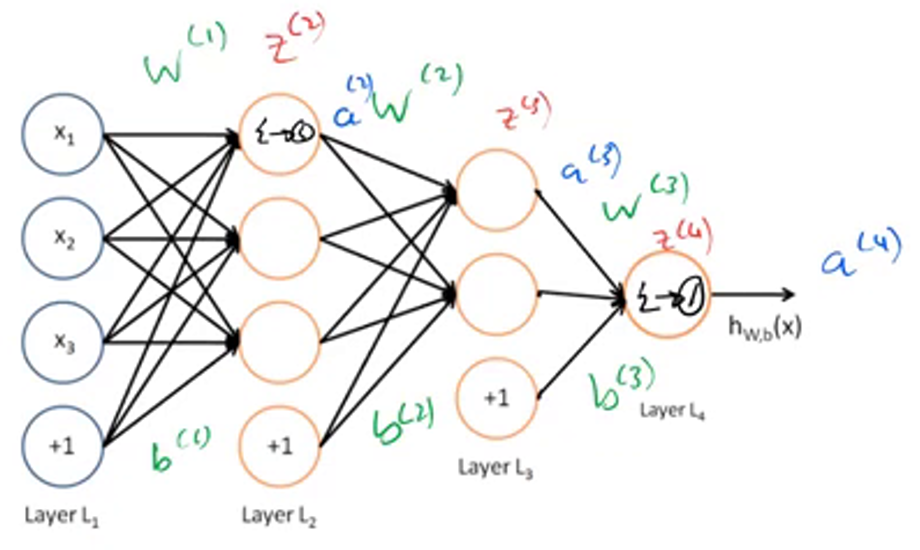
\includegraphics[width=0.5\linewidth]{./images/4layerNN.png}
				\label{fig:nn}
			\end{center}
		\end{figure}
		
		\begin{center}
			Figure \ref{fig:nn}: 4-layer NN representation
		\end{center}
		
		
		
		\subsection{Backprop}
			\subsubsection{Defining the layers and their error contributions}
				\textnormal{Consider a NN for regression with sigmoid activation functions}
			
				\begin{align}
					a^{(l)} &=  f(z^{(l)})\\
					z^{(l)} &= W^{(l-1)} \cdot a^{(l-1)} + b^{(l-1)}
				\end{align}
				
				
				\textnormal{The cost function is:}
				
				\begin{align}
				J(\theta) &= \frac{1}{2}(y - h(x) )^2 \\
				&= \frac{1}{2}(y - a^{(nl)} )^2
				\end{align}
	
							
				\textnormal{where $nl$ is the output layer. To calculate the weight updates of each layer we need to find out how much error each node in those layers contributes.}
				\textnormal{For the output layer we can denote it's error fraction as $\delta^{nl}$ and derive it:}
				
				\begin{align}
					\delta^{(nl)} &= \frac{\partial J(\theta)}{\partial a^{(nl)}}  \odot \frac{\partial a^{(nl)}} {\partial z^{(nl)} }
				\end{align}
				\newpage
				\textnormal{For a hidden layer $l$, we find the error contribution term (gradient) by taking the upstream layer gradient $(l+1)$ and multiply it by the  local gradient. In this way the error portions propagate back through the graph}
				
				\begin{align}
					\delta^{(l)} &= (\delta^{(nl)} \cdot \frac{\partial z^{(l+1)}} {\partial a^{(l)} }) \odot \frac{\partial a^{(l)}} {\partial z^{(l)} }\\
					\delta^{(l)} &= ( \delta^{(nl)} \cdot (W^{(l)})^T ) \odot \frac{\partial a^{(l)}} {\partial z^{(l)} } 
				\end{align}
				
				\textnormal{Remembering that the gradient with respect to a variable should have the same shape as the variable (as each element of that variable is quantifying how much error is being contributed)}
			
			\subsubsection{Algorithm (Batch GD)}
				\begin{enumerate}
					\item Compute a forward pass of the network with the input data, storing the intermediate node values $a^{(l)}$.
					\item Calculate the error term at the output $\delta^{(nl)}$
					\item For each layer $l$ calculate its error term $\delta^{(l)}$
					\item Updating the weights:
						\begin{enumerate}
							\item Find the partials: $\Delta W^{l} = \delta^{(l+1)} \cdot \frac{\partial z^{(l+1)}} {\partial w^{(l)} }$
							\item Update weights: $W^{(l)} = W^{(l)} - \eta (\frac{1}{N}) \Delta W^{l}$
						\end{enumerate}
					\item Updating the biases:
						\begin{enumerate}
							\item Find the partials: $\Delta b^{l} = \delta^{(l+1)} \cdot 1$
							\item Update bias: $b^{(l)} = b^{(l)} - \eta (\frac{1}{N}) \Delta b^{l}$
						\end{enumerate}
				\end{enumerate}
				\textnormal{This can be converted to stochastic GD by adjusting the $\frac{1}{N}$ term in the updates}
				
			
\end{document}